\chapter{Alignment of the SciFi}
\label{sec:story}

% I'd like you to think about the work you have been doing on the alignment and what things have been investigated and what conclusions you have made. You want to build the story one piece at a time, so I think it will start with testing some of the constraints from the null tests and going from there. With the type of work you have been doing, you will also have a much larger "future work" and "continuing work" section, I would put it before the conclusion. This will be discussing things like the way we discovered the cluster bias and the way that it is linked to the rotational degrees of freedom, etc. And it can outline the things you know about the way the real detector will be aligned starting very soon.

% \begin{itemize}
%   \item testing some of the constraints from the null tests
%   \item future work: discovered cluster bias + link to rotational degrees of freedom
% \end{itemize}

% taking notes for now so i know what plots to use
% \begin{enumerate}
%   \item started with null tests.
%   \item which constraint does what?
%   \item which degree of freedom moves what part of the scifi?
% \end{enumerate}

The alignment is performed using run2 data as well as Monte Carlo samples.
The goal is to find the optimal configuration for the SciFi to mirror the real detector.
A configuration is defined as a set of constraints, degrees of freedoms and aligneble objects such as the stations, layers, halflayers, modules or fibre mats.
The following pre-installed alignment conditions with the survey constraints are used.\\

\begin{lstlisting}[language=Python]
  FT : 0 0 0 0 0 0 : 1 1 1 0.0003 0.0003 0.0003
  FT/T. : 0 0 0 0 0 0 : 1 1 1 0.0003 0.0003 0.0003
  FT/T./Layer(X1|U|V|X2) : 0 0 0 0 0 0 : 0.2 0.2 0.2 0.0001 0.0001 0.0001
  FT/.*Module. : 0 0 0 0 0 0 : 0.1 0.1 0.1 0.001 0.001 0.001
  FT/.*Mat. : 0 0 0 0 0 0 : 0.05 0.05 0.05 0.1 0.1 0.1
\end{lstlisting}

The string is the name of the element, the first set of six numbers are hardcoded parameters for each of the 3 translation degrees of freedom and 3 rotational degrees of freedom (Tx, Ty, Tz, Rx, Ry, Rz) and the second set of six parameters are the corresponding uncertainties.

The scale for the translations are $\si{\milli\metre}$ and the scale for the rotations being $\si{\radian}$. A survey uncertainty of $\num{0.0001}$ stands for $\SI{0.1}{\milli\radian}$.

The alignment runs were performed with alignment specific packages from Alignment/Escher and Alignment/TAlignment\cite{align}.

During the alignment, lagrange constraints can be utilized to minimize alignment
parameter $\alpha $ under the condition
\begin{equation}
  f(\alpha) = 0
\end{equation}
and adding the lagrange parameter $\lambda$ to get
\begin{equation}
  \Delta \chi^2 = \lambda f(\alpha)\,.
\end{equation}

Lagrange constraints are added to fix losely constrained degrees of freedom and can be used for any linear combination of translations and rotations.

\section{Nulltests and software tests}

As a starting point, the Alignment version v17r1 was used with 5000 events, magnet in upward position and \textit{GoodLongTracks}.
The \textit{GoodLongTracks} have the following cuts and parameters:
\begin{itemize}
  \item $P_{\text{total, min}} = \SI{5000}{\mega\electronvolt}$ %(units? 5000 MeV?)
  \item $P_{\text{total, max}} = \SI{200000}{\mega\electronvolt}$ %(units? 200 000 MeV = 200 GeV?)
  \item $p_{T, min} = \SI{200}{\mega\electronvolt}$ %(units?)
  \item maximum $\chi^2 = 5$
  \item track type should be categorized as "long"
\end{itemize}

and for the later used \textit{HighMomentumTTracks} the cuts and parameters are:

\begin{itemize}
  \item $P_{\text{total, min}} = \SI{50000}{\mega\electronvolt}$
  \item track type should be categorized as "TTrack"
  \item maximum $\chi^2 = 5$
\end{itemize}

\begin{figure}
  \centering
  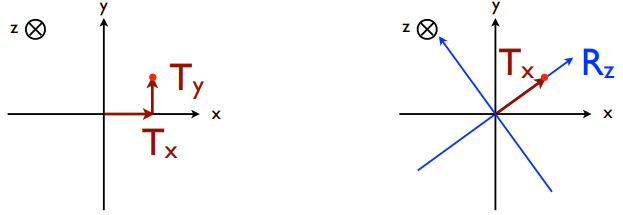
\includegraphics[width=0.75\textwidth]{plots/point_dofs.png}
  \caption{Different ways of describing a measurement point inside the detector(draw this again).}
  \label{fig:dofs}
\end{figure}

At first, a series of tests regarding different degrees of freedom and lagrange constraints is performed to find the optimal solution for the SciFi.

The real detector layers are all centered around the beam pipe with no shifting
in any direction and the goal is to align the layers in the software to mirror
the real layers and reduce the shifting as close to zero as possible.

Figure \ref{fig:dofs} is used to demonstrate which degrees of freedom can be used
to describe a point in the detector or a shift in coordinates.
On the left-hand side the measurement point is described through cartesian coordinates and on the right-hand side it is described via polarcoordinates in a way.

The starting point of the analysis was the presentation held by Florian
Reiss\cite{flo} which contained findings about malfunctioning shearing constraints.
His analysis was performed with the VELO but the ideas are applicable for the SciFi as well.
The parameters he used were changed to fit the SciFi and resulted in

\begin{lstlisting}[language=Python]
    dofs = "TxTyRxRy"
    elements.FTStations(dofs)
    elements.FTFrameLayers(dofs)
    TrackSelections = GoodLongTracks()
\end{lstlisting}\,.

The dataset used is \textit{upgrade\_DC19\_01\_MinBiasMU} taken from the testfileDB\cite{testDB} and will be used for the upcoming tests until a different set is mentioned.
The alignable objects are the (T-)stations and te layers and the trackselection is chosen to be \textit{GoodLongTracks} as a starting point. This will be called \textit{baseline}\footnote{or baseline configuration}.
The baseline is unconstrained in order to see what the software geometry of the detector is like before the alignment with constraints.

In this part, the steps of testing different configurations is described and analysed.

Starting of with the first configuration called "noRotation" tested against the baseline as seen in figure\ref{fig:june_2} for 1000 simulated events used in this particular alignment run and \ref{fig:june_2_1} for 7000 simulated events respectivley.

The measurement points are the mean of each layer, the errorbars are root-mean-square errors (RMS) and come from the difference between the C-side and the A-side of the detector layer and is not the measurement uncertainty.

The "noRotation" configuration is defined as:

\begin{lstlisting}[language=Python]
    dofs = "TxTz"
    elements.FTStations(dofs)
    elements.FTFramelayers(dofs)
    TrackSelections = GoodLongTracks()
    constraints = [
        "station1 : FT/T1 : Tx Tz",
        "station2 : FT/T2 : Tx Tz",
        "station3 : FT/T3 : Tx Tz",
        "frontCSide : FT/T3/Layer(X1|U)/Quarter(0|2) : Tx Tz",
        "backCSide  : FT/T3/Layer(V|X2)/Quarter(0|2) : Tx Tz",
        "frontASide : FT/T3/Layer(X1|U)/Quarter(1|3) : Tx Tz",
        "backASide  : FT/T3/Layer(V|X2)/Quarter(1|3) : Tx Tz"
    ]
\end{lstlisting}

Here, only x-translation will be compared since other translatory degrees of freedom will be swapped out for a rotational degree of freedom (DoF).
The first three constraints on all stations regarding translations brings the total movement of the station to around zero which can be seen clearly in figure\ref{fig:june_2}. The last four constraints restrict the movement of each
side of the C-frame to be centered around zero which brings the x translation in station 3 even closer to zero.
Even though the alignment improved the amount of constraints cannot recover from potential misalignments because the constraints hinder the stations from moving.

Later on we want as few constraints as possible so that the alignable objects can be aligned and converge towards the optimal position based on the track reconstruction.
This measurement only used 1000 events and is only used as a guideline to what the trend of the distribution looks like. The associated graphs for $Tx$ plotted against the group position in $z$ are shown in figure \ref{fig:june_2}.
A prominent problem visible is the layer separation between the X-layers and the stereo layers as well as a separation between the C-frames inside each station.

\begin{figure}
  \centering
  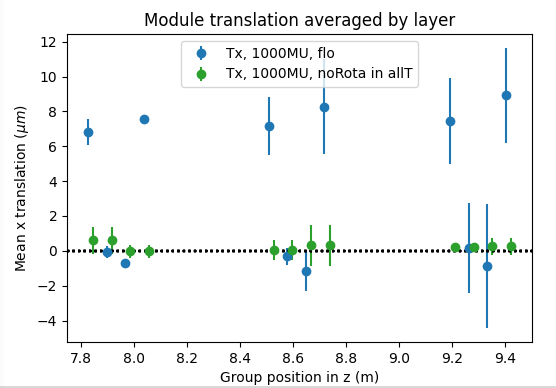
\includegraphics[width=0.8\textwidth]{plots/june_21/Tx_noRota_allT_1000MU.png}
  \caption{comparison of different configurations without rotational constraints in every station, magnet up and 1000 events. plotted is translation in x versus global z.}
  \label{fig:june_2}
\end{figure}

\begin{figure}
  \centering
  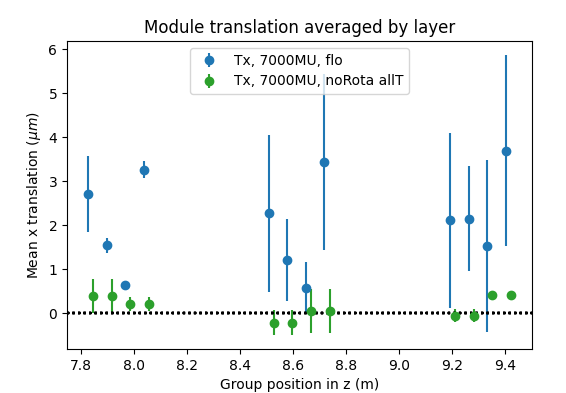
\includegraphics[width=0.8\textwidth]{plots/june_21/Tx_noRota_allT_7000MU.png}
  \caption{comparison of different configurations without rotational constraints in all stations, magnet up and 7000 events. plotted is x translation versus global z.}
  \label{fig:june_2_1}
\end{figure}

In figure \ref{fig:june_2_1} the same measurement was performed for 7000 events to get a better picture. In comparison to \ref{fig:june_2} an overall improvement of the baseline is visible and the layer-splitting is reduced but still prominent. The green measurement shows no direct improvement since the layers are already pretty close to zero in x-direction.
Using 7000 events instead of 1000 events showed a more realistic picture but
took more time to compute especially for 10 alignment iterations.
For the following configuration, 3000 simulated events were used to shorten the computing time while still yielding an accurate representation of the situation.

% for comparisons include the 3000MU plot from renewed_plots

The next configuration tested will be called "half C-frame". This configuration is defined as

\begin{lstlisting}[language=Python]
    dofs = "TxTzRxRz"
    elements.FTStations(dofs)
    elements.FTFramelayers(dofs)
    TrackSelections = GoodLongTracks()
    constraints = [
        "station1 : FT/T1 : Tx Tz",
        "station2 : FT/T2 : Tx Tz",
        "station3 : FT/T3 : Tx Tz",
        "frontCSide : FT/T3/Layer(X1|U)/Quarter(0|2) : Tx Tz : total",
        "backCSide  : FT/T3/Layer(V|X2)/Quarter(0|2) : Tx Tz : total"
]
\end{lstlisting}

and the comparison to the baseline is shown in figure \ref{fig:june_3}.
Here the stations and layers are aligned in $Tx$, $Tz$, $Rx$ and $Rz$ but the stations are still only constrained in their translations. Also, the last station only has one side of each C-frame constrained. The additional keyword \textbf{total} constraints
the difference of the quarters to zero with respect to the nominal position. As seen in figure \ref{fig:june_3} the first two layers have an average position of zero but the individual position is not. The same is seen in the last two layers of each station.

This new configuration in orange converged after 12 iterations as seen in figure \ref{fig:conv}. Normally, an alignment job should converge after three to five iterations. If the convergence happens later there could be a problem with the constraints which prevent the alignment from converging because they are implemented wrongly, are redundant or weak modes hinder the convergence.

\begin{figure}
  \centering
  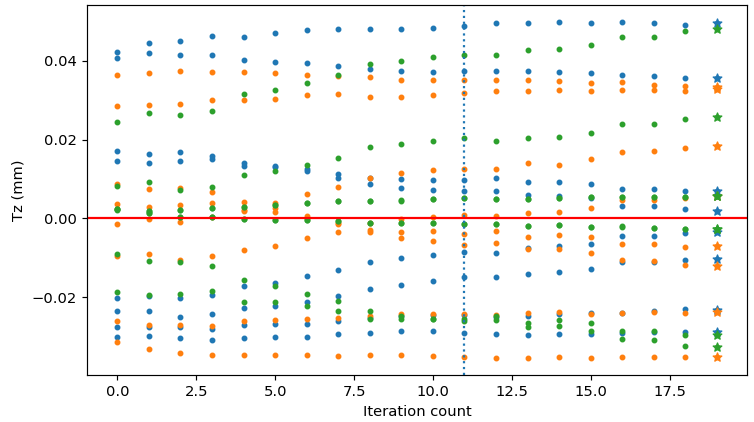
\includegraphics[width=0.5\textwidth]{plots/scatter_fig_4_4_convergence.png}
  \caption{convergence after 12 iterations from configuration "half C-frame".}
  \label{fig:conv}
\end{figure}

\begin{figure}
  \centering
  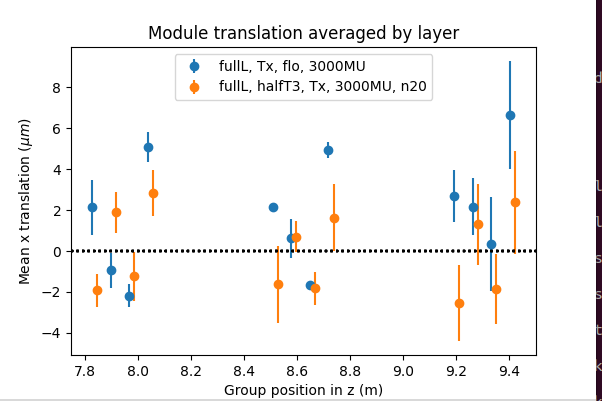
\includegraphics[width=0.8\textwidth]{plots/june_21/allT_halfT3_n20_Tx.png}
  \caption{analysed 20 iterations for x translation behavior for configuration "half C-frame".}
  \label{fig:june_3}
\end{figure}

\section{rotational constraints}
In the previous section rotations were not used inside the constraints. Now the constraints will include rotational constraints and test the changes.

Similar to the "noRotation" configuration the same constraints were used but for different degrees of freedom. The new configuration is called "Full DoF" which uses every degree of freedom and is defined as:

\begin{lstlisting}[language=Python]
    dofs = "TxTyTzRxRyRz"
    elements.FTStations(dofs)
    elements.FTFramelayers(dofs)
    TrackSelections = GoodLongTracks()
    constraints = [
        "station1 : FT/T1 : Tx Ty Tz Rx Ry Rz",
        "station2 : FT/T2 : Tx Ty Tz Rx Ry Rz",
        "station3 : FT/T3 : Tx Ty Tz Rx Ry Rz",
        "frontCSide : FT/T3/Layer(X1|U)/Quarter(0|2) : Tx Ty Tz Rx Ry Rz",
        "backCSide  : FT/T3/Layer(V|X2)/Quarter(0|2) : Tx Ty Tz Rx Ry Rz",
        "frontASide : FT/T3/Layer(X1|U)/Quarter(1|3) : Tx Ty Tz Rx Ry Rz",
        "backASide  : FT/T3/Layer(V|X2)/Quarter(1|3) : Tx Ty Tz Rx Ry Rz"
        ]
\end{lstlisting}

In figure \ref{fig:june_4} x-translation and z-translation with regards to
the group position are shown.

\begin{figure}
  \centering
  \begin{subfigure}[b]{0.4\textwidth}
    \centering
    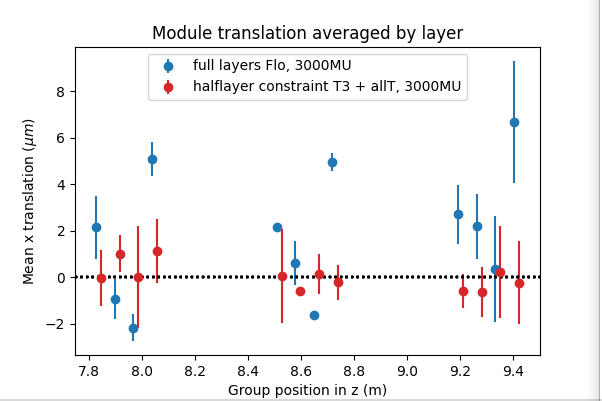
\includegraphics[width=\textwidth]{plots/june_21/allT_halfT3_Tx_vs_Flo.png}
    \caption{x-translation versus group position in z.}
    \label{fig:june_4_1}
  \end{subfigure}
  \hfill
  \begin{subfigure}[b]{0.4\textwidth}
    \centering
    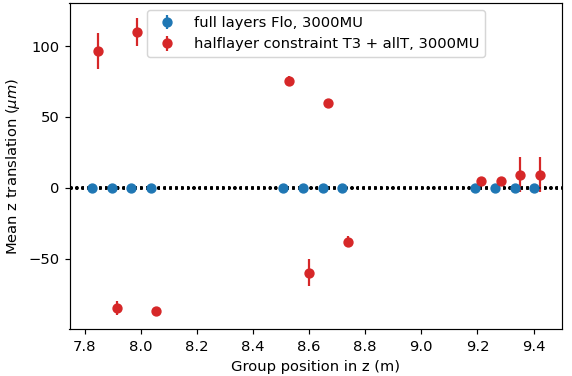
\includegraphics[width=\textwidth]{plots/scatter_fig4_2.png}
    \caption{z-translation versus group position in z.}
    \label{fig:june_4_2}
  \end{subfigure}
  \caption{"Full DoF" configuration (red) plotted versus baseline configuration (blue) for 3000 events.}
  \label{fig:june_4}
\end{figure}

Figure \ref{fig:june_4_1} still shows layer separation in station 1 more similar to figure \ref{fig:june_3} than to figure \ref{fig:june_2_1}.
Since the constraints are the same and the amount of degrees of freedoms increased,
it is visible that using more DoFs makes the alignment worse. Therefore the degrees of freedom must be chosen wisely.

Regarding the z-translation the plot is only shown to demonstrate the large separation of layers. the baseline was not aligned in $Tz$ so there is no comparison.
% Will do an alignment run to get it!
The RMS uncertainty on the measurements is a result of the separation between A-side and C-side. For configuration "Full DoF", a plot showing the C-side and A-side difference in x-translation is shown in figure \ref{fig:june_5} and for z-translation in figure \ref{fig:june_6}.

A clear layer separation is visible in terms af layer translation along the beam pipe\ref{fig:june_5}.
The first and third layer in each station move away from the IP and the second and
fourth layer move towards the IP.
Because of the many constraints that are applied to T3, the RMS uncertainty in the other stations get worse. Because the last station is overconstrained the track reconstruction moves the other stations accordingly which results in a larger RMS uncertainty in station 1 and 2.

\begin{figure}
  \centering
  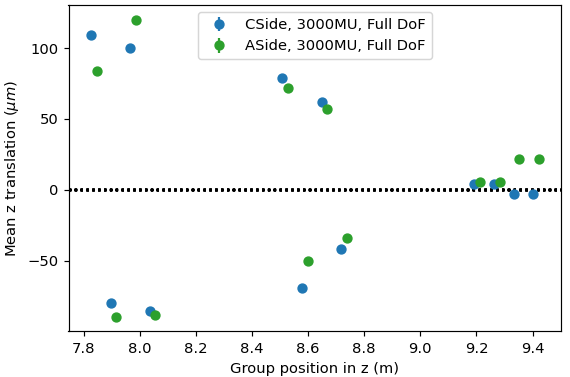
\includegraphics[width=0.8\textwidth]{plots/renewed_plots/CA_allT_halfT3_Tz.png}
  \caption{compare C-Side to A-Side for translation in z direction.}
  \label{fig:june_5}
\end{figure}
On the other hand the x-translation \ref{fig:june_6}
\begin{figure}
  \centering
  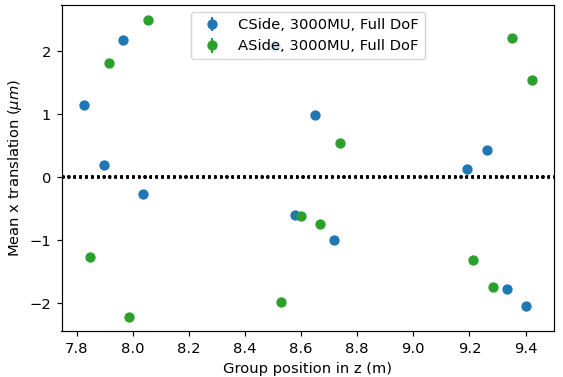
\includegraphics[width=0.8\textwidth]{plots/renewed_plots/CA_allT_halfT3_Tx.png}
  \caption{compare C-Side to A-Side for translation in x direction.}
  \label{fig:june_6}
\end{figure}

Looking at figure \ref{fig:june_6}, the last two layers in station 3 are
seperated from the first two regarding x-translation. Especially the last
station should be fixed around zero with the constraints added. The sum of
all translations should be zero with each individual layer movement being small.

The result is unexpected with the constraints added and the cause of this
problem is described later.

The Next configuration tested is the result of a series of tests with various constraints, DoFs and alignable objects. In figure \ref{fig:TxZ} a new configuration called "Test3" is introduced and it is defined as

\begin{lstlisting}[language=Python]
dofs = "TxTzRxRz"
elements.FTStations(dofs)
elements.FTFramelayers(dofs)
TrackSelections = GoodLongTracks()
constraints = [
    "station3 : FT/T3 : Tx Tz Rx Rz",
    "frontCSide : FT/T3/Layer(X1|U)/Quarter(0|2) : Tx Tz Rx Rz",
    "backCSide  : FT/T3/Layer(V|X2)/Quarter(0|2) : Tx Tz Rx Rz",
    "frontASide : FT/T3/Layer(X1|U)/Quarter(1|3) : Tx Tz Rx Rz",
    "backASide  : FT/T3/Layer(V|X2)/Quarter(1|3) : Tx Tz Rx Rz"
    ]
\end{lstlisting}
% test 3:

\begin{figure}
  \centering
  \begin{subfigure}[b]{0.4\textwidth}
    \centering
    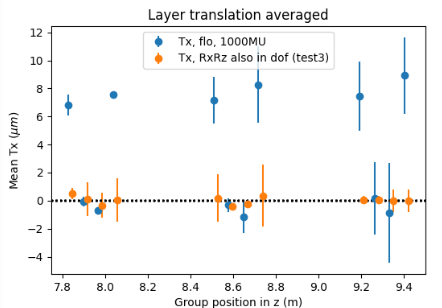
\includegraphics[width=\textwidth]{plots/july_28/Tx.png}
    \caption{x-translation versus group position in z.}
    \label{fig:TxZ_1}
  \end{subfigure}
  \hfill
  \begin{subfigure}[b]{0.4\textwidth}
    \centering
    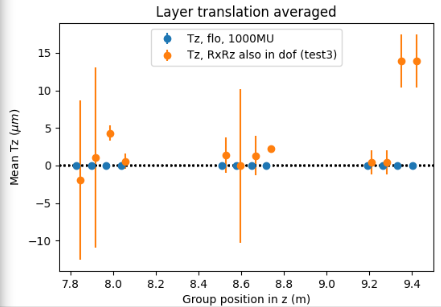
\includegraphics[width=\textwidth]{plots/july_28/Tz.png}
    \caption{z-translation versus group position in z.}
    \label{fig:TxZ_2}
  \end{subfigure}
  \caption{"Test3" configuration (orange) plotted versus baseline configuration (blue) for 1000 events.}
  \label{fig:TxZ}
\end{figure}

Here the last four C-frame constraints have rotational degrees of freedom added.
Looking at \ref{fig:TxZ_1} each station has a quite low movement in x-direction comparing to the previous configurations. In the last station, the first two layers the C-side and A-side are exactly where they should be inside the detector since the RMS is very close to zero. The last two layers only show a small uncertainty. In station
two the X-layers are separating from the stereolayers. The X-layers also have a noticable RMS uncertainty. In this configuration the degrees of freedom are chose in a way for the alignment to either use them as two pairs of cartesian coordinates (Tx Tz, and Rx Rz) or interpret them as two pairs of polar coordinates (Tx Rz and Tz Rx).
This and also the reduction in constraints seemed to help the alignment in terms of x-translation, not so much regarding z-translation. Also this plot only shows the alignment for 1000 events and 10 iterations but overall an improvement was achieved
when it comes to constructing a good configuration.

The next configurations are called "config5" (blue) and "config5 Rz" (orange). The plots showing the translations are shown in figure \ref{fig:config5_tra} and the rotations are shown in figure \ref{fig:config5_rot}.
The blue measurement has the same constraints as "Test3" with an added back C-frame constraint:
\begin{lstlisting}[language=Python]
  constraints.append("back_C_frame_T3 : FT/T3/Layer(V|X2) : Tx Tz")
\end{lstlisting}

The orange measurement has a similar constraint added with Rz added to the DoFs inside the constraint:
\begin{lstlisting}[language=Python]
  constraints.append("back_C_frame_T3 : FT/T3/Layer(V|X2) : Tx Tz Rz")
\end{lstlisting}

Comparing just these two configurations, regarding $Tx$ there is not a big difference.
The last station has a little more separation in "config5 Rz", station 2 shows roughly the same performance and station one is also more split, in total approximately
$\SI{0.5}{\micro\metre}$. The overall z-translation regressed by a small amount in every station while the layer spearation in station 3 improved.
It can be sen, that both X-layers in T2 in the x-translation plot have a quite large RMS uncertainty which means the A-side and the C-side in the X-layers are quite far apart but the mean is right around 0. That is expected since the constraint added only brings the mean of the layer to 0. In future analyses new constraints will be added to bring the sides together.
% config 5
\begin{figure}
  \centering
  \begin{subfigure}[b]{0.4\textwidth}
    \centering
    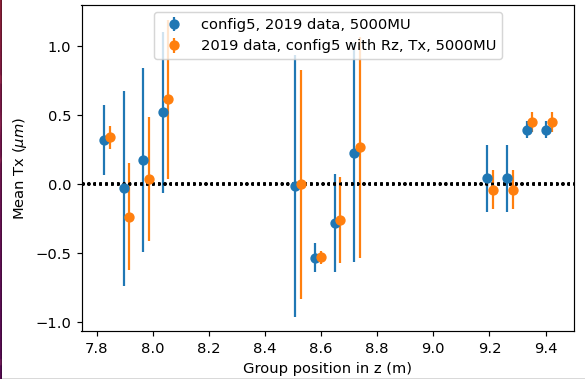
\includegraphics[width=\textwidth]{plots/renewed_plots/Tx.png}
    \caption{x-translation versus group position in z.}
    \label{fig:config5_Tx}
  \end{subfigure}
  \hfill
  \begin{subfigure}[b]{0.4\textwidth}
    \centering
    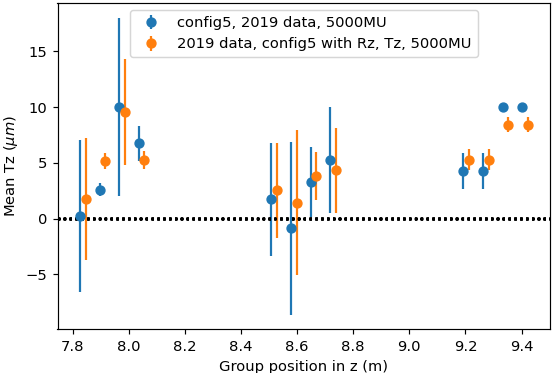
\includegraphics[width=\textwidth]{plots/renewed_plots/Tz.png}
    \caption{z-translation versus group position in z.}
    \label{fig:config5_Tz}
  \end{subfigure}
  \caption{"config5" configurations (blue) plotted versus "config5 Rz" configuration (orange) for 5000 events.}
  \label{fig:config5_tra}
\end{figure}

Rotations around $x$ will not be further analysed because it does not have a huge impact on the alignment quality and is also very well aligned. In $Rz$ a noticable gap
between the two measurements can be seen. This is a result from the added $Rz$
constraint on the last two layers. The expected rotation is small than shown in figure \ref{fig:config5_Rz} which is expected to be a result from bias in the clusters.

\begin{figure}
  \centering
  \begin{subfigure}[b]{0.4\textwidth}
    \centering
    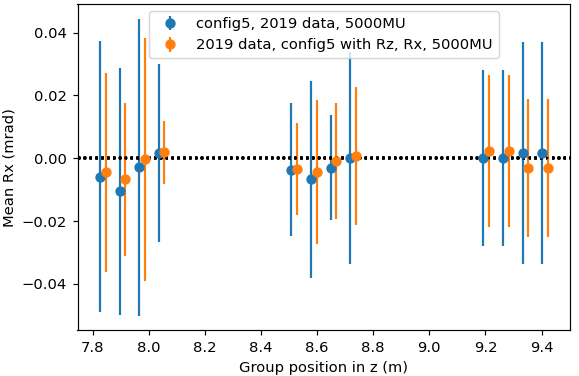
\includegraphics[width=\textwidth]{plots/renewed_plots/Rx.png}
    \caption{x-rotation versus group position in z.}
    \label{fig:config5_Rx}
  \end{subfigure}
  \hfill
  \begin{subfigure}[b]{0.4\textwidth}
    \centering
    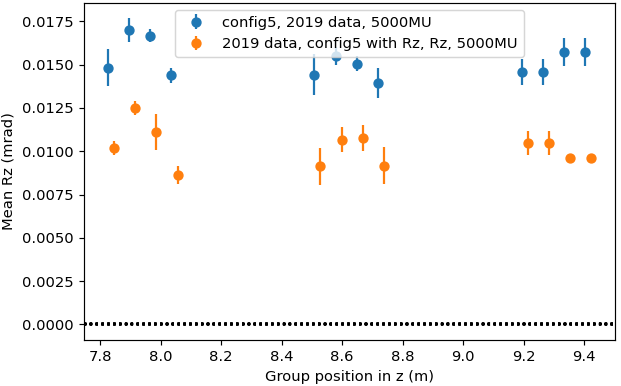
\includegraphics[width=\textwidth]{plots/renewed_plots/Rz.png}
    \caption{z-rotation versus group position in z.}
    \label{fig:config5_Rz}
  \end{subfigure}
  \caption{"config5" configurations (blue) plotted versus "config5 Rz" configuration (orange) for 5000 events.}
  \label{fig:config5_rot}
\end{figure}

Regarding the goal to reduce the amount of rotation and translation in each station,
the result is a small improvement in $Rz$ of around $\SI{0.005}{\milli\radian}$ in every layer. $Rx$ is mostly unchanged aswell as $Tx$.

% \begin{figure}
%   \centering
%   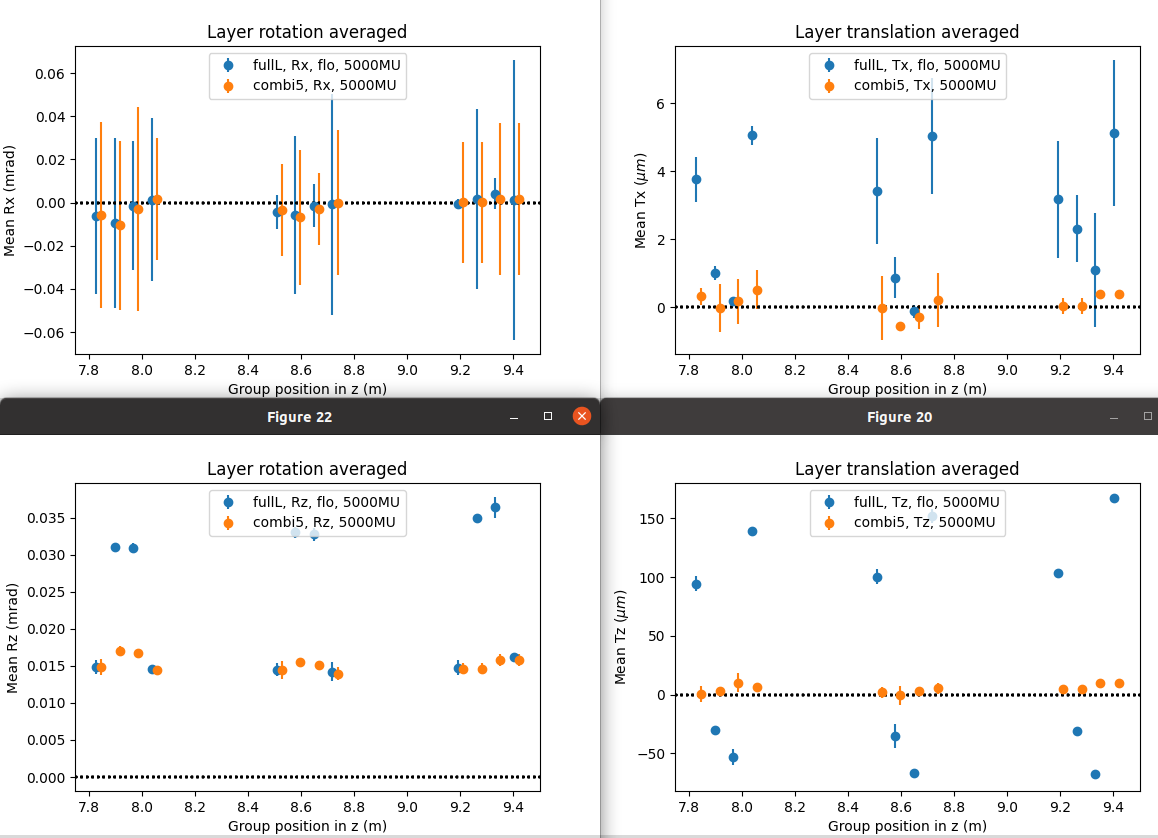
\includegraphics[width=0.8\textwidth]{plots/august_13/combi5_layers_averaged.png}
%   \caption{flo with full layer constraint versus config 5}
%   \label{fig:floFullL_c5}
% \end{figure}

% In comparison to the baseline against the new proposed configuration the figure \ref{fig:floFullL_c5} can be looked at.
% The alignment was performed for 10 iterations and the alignable degrees of
% freedom are $\symup{Tx}, \symup{Tz}, \symup{Rx}, \symup{Rz}$. The alignable
% elements are the stations and the framelayers.
% The constraints used are: \\
%
% \begin{lstlisting}[language=Python]
%   station3 : FT/T3 : Tx Rz Rx Rz
%   backCframeT3 : FT/T3/Layer(V|X2) : Tx Tz
%   FT/T3X1UCSide : FT/T3/Layer(X1|U)/Quarter(0|2) : Tx Tz Rx Rz
%   FT/T3VX2CSide : FT/T3/Layer(V|X2)/Quarter(0|2) : Tx Tz Rx Rz
%   FT/T3X1UASide : FT/T3/Layer(X1|U)/Quarter(1|3) : Tx Tz Rx Rz
%   FT/T3VX2ASide : FT/T3/Layer(V|X2)/Quarter(1|3) : Tx Tz Rx Rz
% \end{lstlisting}

% The first constraint restricts the overall station 3 movement in $\symup{Tx}, \symup{Tz},
% \symup{Rx}$ and $\symup{Rz}$. The second constraint restricts the total movement
% of the last C-frame to be 0 but the individual movement can differ.
% The last four constraints are C-frame constraints as well but for each halflayer in station 3.
%
% It is good to see that the layer separation in $Rz$ is mostly fixed. But there is still an offset from 0 that is troublesome. This will most certainly have something to do with the clusterbias. Regarding $Tx$, we have managed to bring down the x-translation to roughly 0 which is a good improvement for the null tests of $Tx$.

Translation constraints as well as rotation constraints are not the only constraints tested. There are also scaling- and shearing constraints that were analysed but seemed to have no major impact.


% november plots
\section{chi2 tests and weak modes}
In this section, a $\chi^2$ analysis is performed in order to study the "goodness" of the alignment since the better the $\chi^2$ after the alignment the better.
The second aspect i want to cover is the impact of potential weak modes also known as "correlated alignment parameters". There are several weak modes that could occur namely \textit{global translation}, \textit{shearing} and \textit{curvature bias}.
Weak modes are unaffected by the $\chi^2$ since the residuals do not change but they do however show inside the eigenvalues of track parameters.
The effect weak modes have on the alignment are biases regarding track parameters and late convergences.
There are different solutions that can be utilized to reduce the effect from weakmodes such as
\begin{itemize}
  \item $\textbf{using other configurations like magnet off or mass plots for off-axis events}$
  \item $\textbf{utilizing other survey data sets}$
  \item $\textbf{using kinematic and vertex constraints}$
\end{itemize}\,.

\begin{figure}
  \centering
  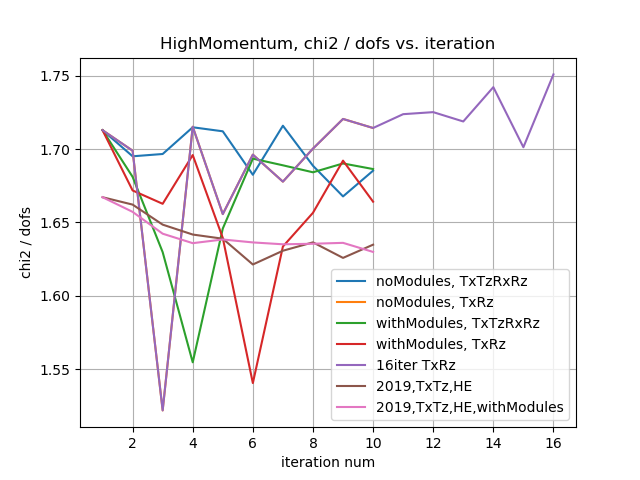
\includegraphics[width=0.8\textwidth]{plots/nov_19/Figure_2.png}
  \caption{$\chi^2 / dofs$ versus iteration number of different degrees of freedom, alignables and data samples.}
  \label{fig:fig2}
\end{figure}

We started with the $\chi^2$-analysis for \textit{HighMomentumTTracks},
6500 events and 2020 data plotted versus the iteration number during the
alignment in figure \ref{fig:fig2}. In blue, stations and layers were aligned in $Tx$,
$Tz$, $Rx$ and $Rz$ with the constraints being used from "config5". The orange
measurement is identical except for the degrees of freedoms being only $Tx$ and $Rz$.
In green and red the same measurements as in blue and orange were performed with
the difference that that the modules are aligned as well.
The purple measurement is the only one which covers 16 iterations and is otherwise identical to the orange one. That is also why the orange measurement is not visible since it lies behind the purple one for the first 10 iterations.
the brown and pink measurements are done for 2019 data and are otherwise identical to the orange and red measurement regarding constraints and alignable degrees of freedom.

The spikey behavior is not what we expected and this might be the result of weak modes since the convergence is quite bad in all of the 2020 data which can be seen by the not
steadily decreasing $\chi^2 / dofs$.
The 2019 measurements were performed as control measurements with and without
module alignment. Here a clear decrease in the $\chi^2 / dofs$ is visible. This
indicates that for the 2020 data additional analysis must be performed to gain further knowledge about the dataset since it shows some unclear findings.

The idea to test $Tx$, $Tz$, $Rx$ and $Rz$ versus only one translation and one
rotational degree of freedom was to analyse the effect regarding the convergence and the $\chi^2 / dofs$ itself. One could also argue that there was a quick convergence after three iterations when looking at the yellow measurement but something happened afterwards. This will be analysed in a future project.

Also, in figure \ref{fig:chi2iter} the same plot is presented but only for the first four measurements clean up the image. The same four $\chi^2$ measurements were plotted
against the number of tracks as seen in figure \ref{fig:chi2tracks}. It is pleasing to see a steady decrease in $\chi^2 / dofs$ with an increasing number of tracks. This was done as a consistency check.

\begin{figure}
  \centering
  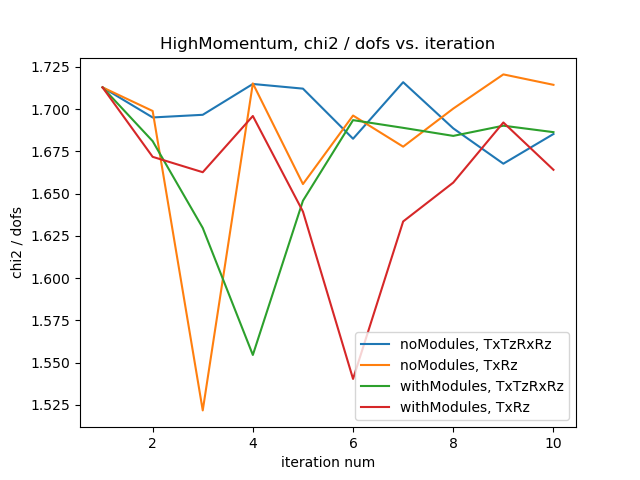
\includegraphics[width=0.8\textwidth]{plots/nov_21/chi2_vs_iter_all.png}
  \caption{$\chi^2$-test versus iteration number of different degrees of freedom, alignables and data samples but fewer (redo with grid).}
  \label{fig:chi2iter}
\end{figure}

\begin{figure}
  \centering
  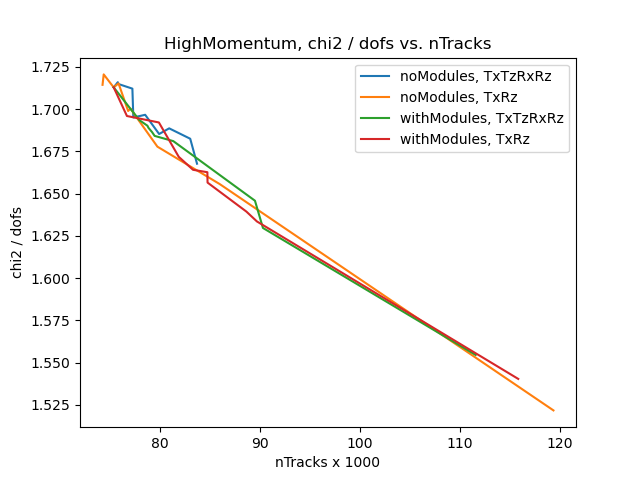
\includegraphics[width=0.8\textwidth]{plots/nov_21/chi2_vs_ntracks_all.png}
  \caption{$\chi^2$-test versus number of tracks of different degrees of freedom, alignables and data samples but fewer (redo with grid).}
  \label{fig:chi2tracks}
\end{figure}

% december plots
\begin{figure}
  \centering
  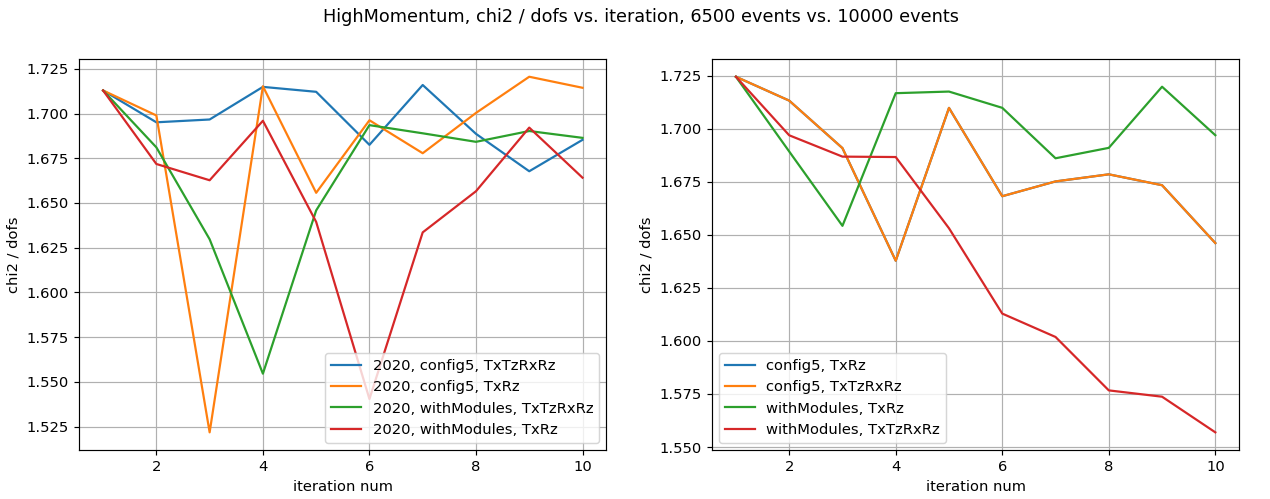
\includegraphics[width=\textwidth]{plots/LHCB_week_dec/chi2_vs_iter_normal.png}
  \caption{$\chi^2 / dofs$ versus iteration number for different number of events.}
  \label{fig:chi2iterdec}
\end{figure}

In figure \ref{fig:chi2iterdec} a side-by-side view of the same $\chi^2$ measurement
is shown but for different number of events. Despite the different labels these are the same measurements, only the colors are switched around for red and green and also yellow and blue as a pair. The thing that strikes the eye is the steadily decrease in $\chi^2 / dofs$ in the red measurement. Unlike our first expectations that $Tx$ and $Rz$ are enough degrees of freedom to describe the system using additional degrees of freedom seemed to help the alignment.
Also, the blue measurement sits behind the orange which might be due to an
programming error.

In figure \ref{fig:chi2tracksdec} a consistency check for figure
\ref{fig:chi2iterdec} was performed. The number of tracks correlate good with
the $\chi^2 / dofs$. The blue measurement is missing again which seems to be a
programming error.

\begin{figure}
  \centering
  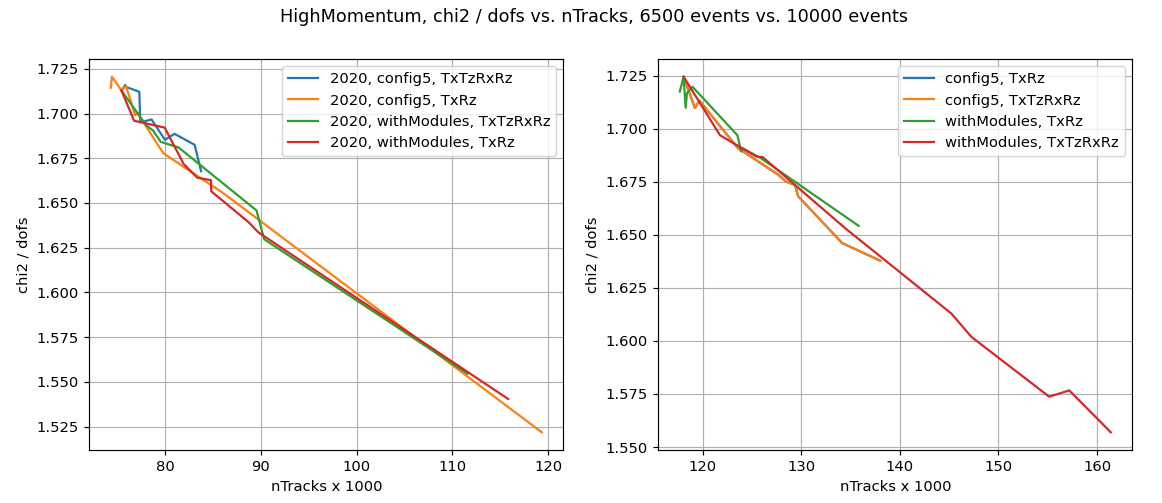
\includegraphics[width=\textwidth]{plots/LHCB_week_dec/chi2_vs_tracks_normal.png}
  \caption{$\chi^2 / dofs$ versus number of Tracks for 6500 events and 10000 events.}
  \label{fig:chi2tracksdec}
\end{figure}

\section{luminosity samples and chi2}
For a cross check regarding upcoming studies the difference in $\chi^2 / dofs$ for samples of different luminosities are looked at.
Comparing two samples, one with a "ramp-up" luminosity with a parameter $\nu = 3.8$ also referred to as "low luminosity" and one for the luminosity used during the data taking
with $\nu = 7.6$, called "normal luminosity".
Plotted are these samples in $\chi^2 / dofs$ versus the iteration number \ref{fig:chi2iter_lumi_normal} and the number of tracks\ref{fig:chi2tracks_lumi_normal}.

in figure \ref{fig:chi2iter_lumi_normal} we see the expected convergence after iteration three and a quite low $\chi^2 / dofs$ of around $\num{1.28595}$ for the normal luminosity sample and $\num{1.3067}$ for the low luminosity sample.

\begin{figure}
  \centering
  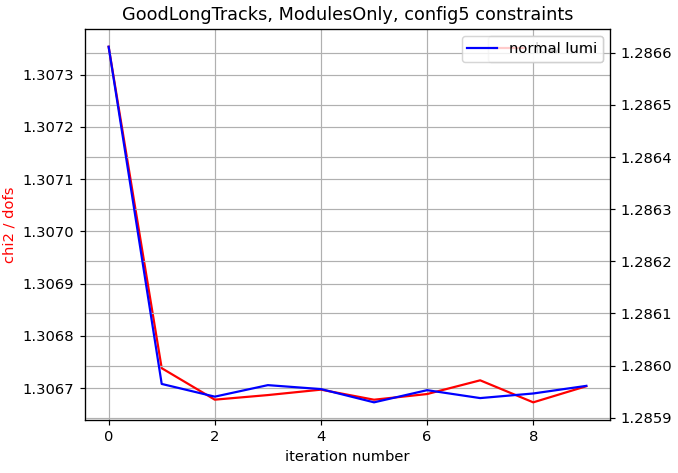
\includegraphics[width=0.8\textwidth]{plots/renewed_plots/modules_chi2_c5.png}
  \caption{compare different luminosities and plot $\chi^2$ versus iteration number.}
  \label{fig:chi2iter_lumi_normal}
\end{figure}

\begin{figure}
  \centering
  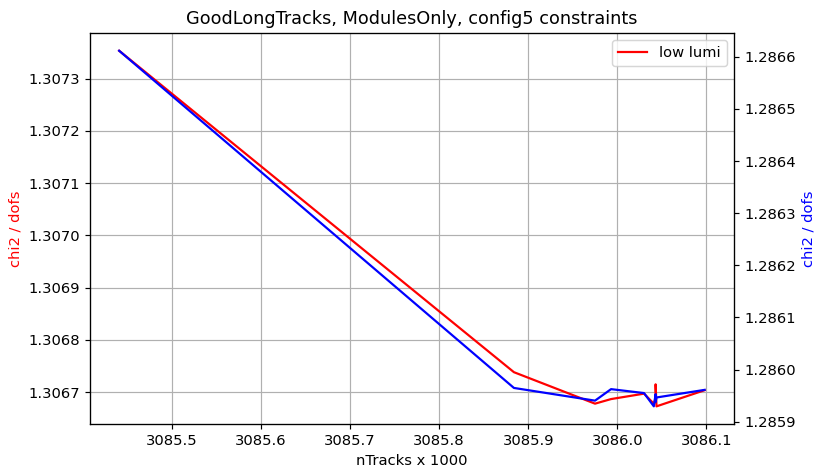
\includegraphics[width=0.8\textwidth]{plots/jan_17_2022/chi2_tracks_modulesOnly.png}
  \caption{compare different luminosities and plot $\chi^2$ versus number of tracks as a measurement for weakmodes and alignment.}
  \label{fig:chi2tracks_lumi_normal}
\end{figure}

\section{impact of the cluster bias}

As mentioned earlier the clusterbias most certainly causes the shift in the rotation around $z$ for each layer so it does not reach 0.
To test that a momentary fix was found and implemented. The workaround was to add a scaling for the \textit{m\_airgap}\cite{gap}.

Figure \ref{fig:cbhack_on_off} shows the impact of the cluster bias fix regarding
the rotation around $z$.

\begin{figure}
  \centering
  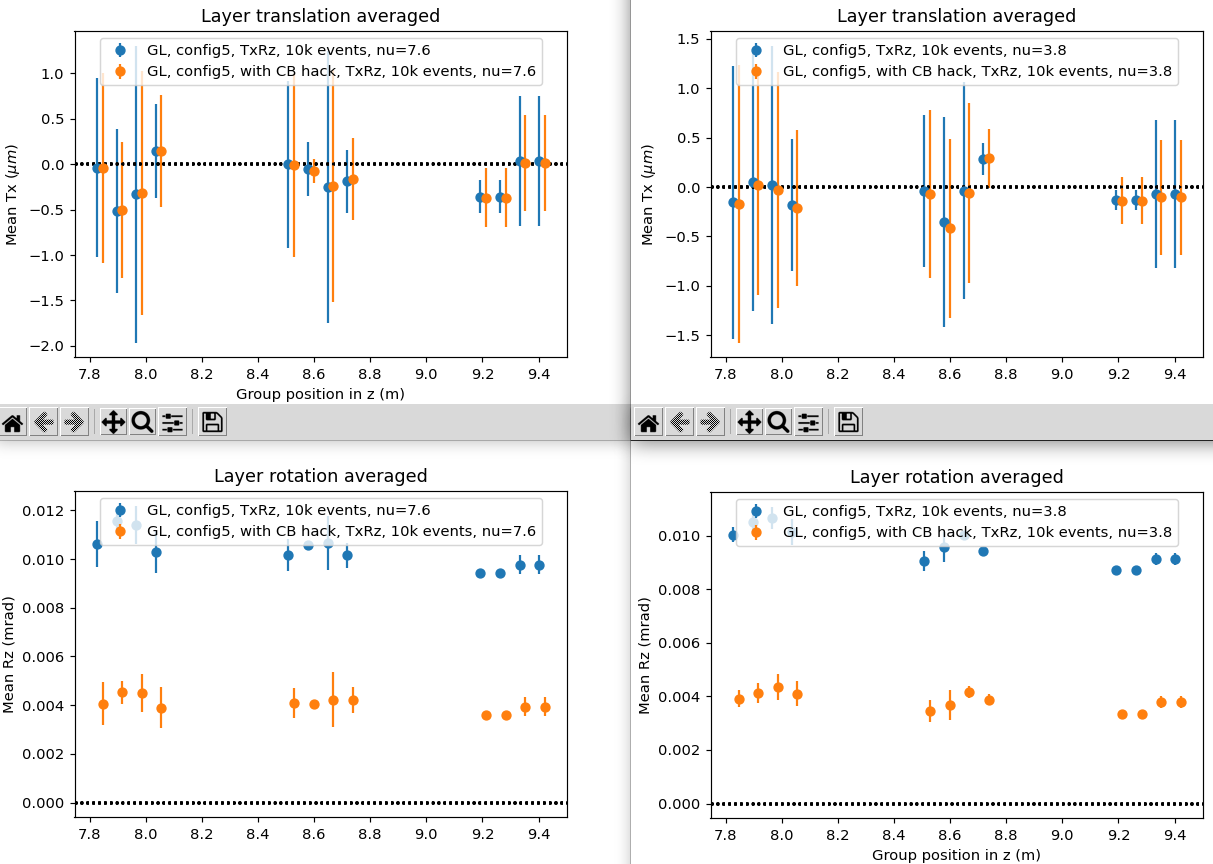
\includegraphics[width=0.8\textwidth]{plots/jan_24_2022/compare_with_without_hack.png}
  \caption{Impact of the clusterbias for high and low luminosity samples.}
  \label{fig:cbhack_on_off}
\end{figure}

As we expected, the amount of rotation was reduced to about
$\SI{0.004}{\milli\radian}$ from the previous $\SI{0.01}{\milli\radian}$ which is more than a factor of 2 improvement. We also know, that the fix for the cluster bias will not be the only source for the shift and we need further analysis to find the other sources.

Now that we know that the cluster bias can be taken care of we take a closer look at samples of different luminosities since the LHC will not be operated at the maximum luminosity from the start, there is also the ramp up phase where the luminosity will be lower.

Since we want to know what the shifts in rotation and translation will look like when the cluster bias is fixed we will keep it active for the next studies.
Figure \ref{fig:lumi_low_normal_hack_on} shows the difference between a sample with ramp-up luminosity and a sample with the luminosity during the measurement phase.
We see, that the layer separation is much more prominent in station 1 and 3 for the higher luminosity sample but slightly better behaved in station 2 when looking at x-translation.
Regarding the z-rotation, the lower luminosity sample as slightly lower rotational shifts.
The difference is so minute that it can be safely disregarded.

\begin{figure}
  \centering
  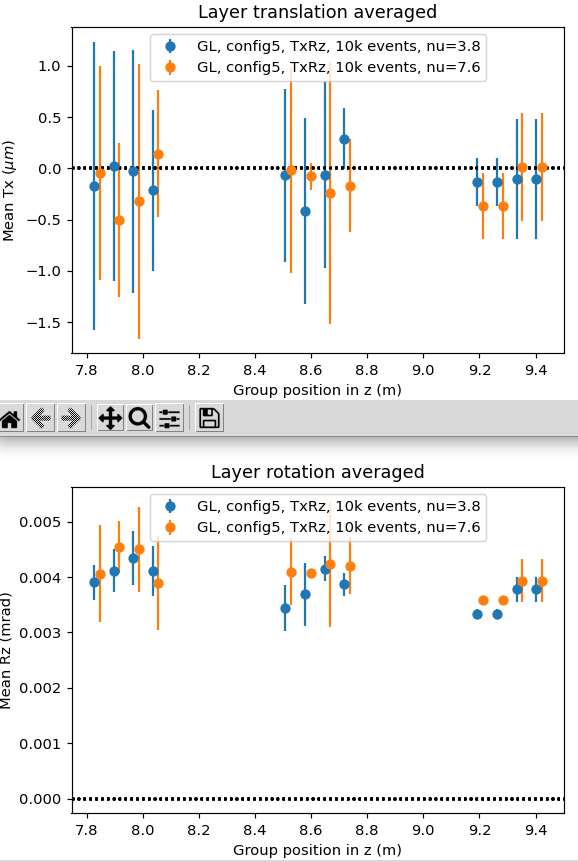
\includegraphics[width=0.8\textwidth]{plots/jan_24_2022/low_normal_with_hack.png}
  \caption{show difference between low and normal luminosity with clusterbias fix active.}
  \label{fig:lumi_low_normal_hack_on}
\end{figure}

With that, we tested if there is a noticable difference in the $\frac{\chi^2}{\text{dof}}$ and the result is shown in figure \ref{fig:GL_lumi_low_normal_hack_on}.

\begin{figure}
  \centering
  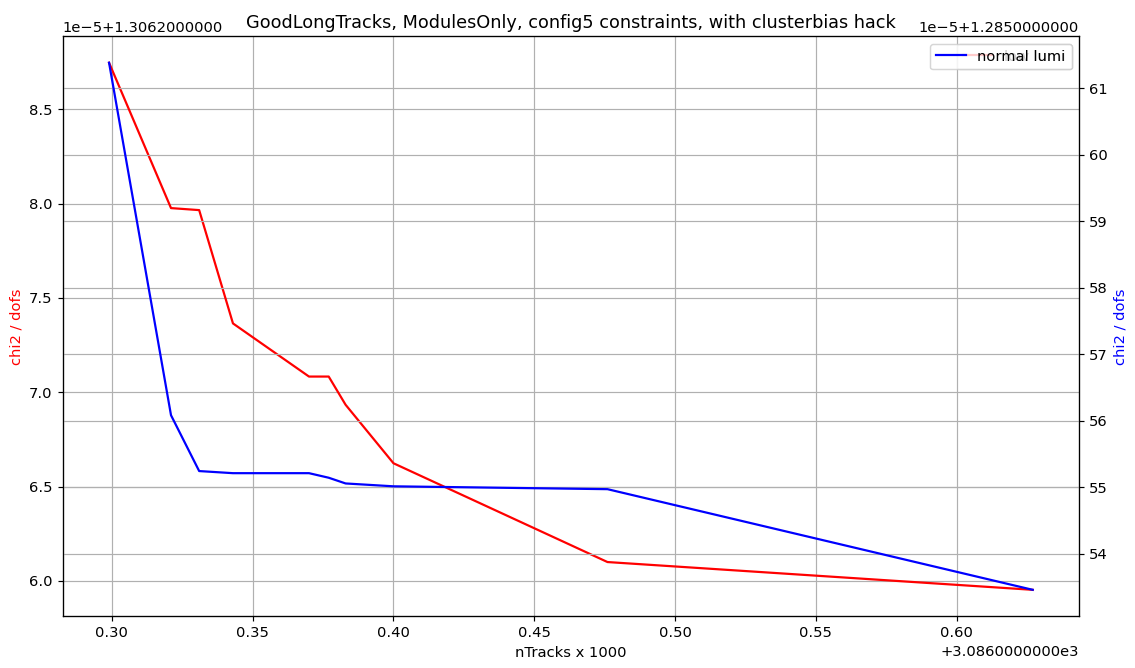
\includegraphics[width=0.8\textwidth]{plots/feb_2_2022/GL_modules_c5_cb_hackactive_low_normal_lumi.png}
  \caption{GoodLong tracks for module alignment and config 5 active. also the clusterbias fix is active comparing low and normal luminosity.}
  \label{fig:GL_lumi_low_normal_hack_on}
\end{figure}

\begin{figure}
  \centering
  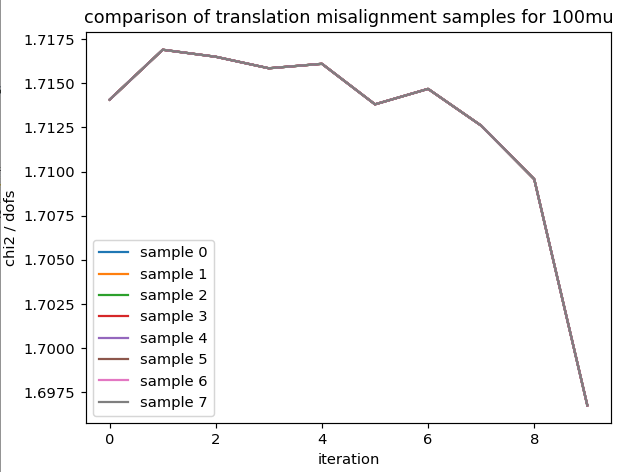
\includegraphics[width=0.8\textwidth]{plots/feb_6_2022/100mu_misalignment_samples_compared.png}
  \caption{100mu translation misalignment comparison for different misalignment samples.}
  \label{fig:100muT}
\end{figure}

Now, since the alignment works quite good with the current configuration we
tested how translation misalignment effects the convergence by looking at the
$\chi^2$, portrayed in figure \ref{fig:100muT}. For this figure, eight different samples of $\SI{100}{\micro\metre}$ module translation misalignment over all translatory
degrees of freedom. The idea behind using different samples is to reduce errors
from biased samples. The plot shows the total $\chi^2$ over degrees of freedom
plotted against the number of iterations. We see no visible difference regarding
the total $\chi^2$ between the samples which is good.
Also, the total $\chi^2$ decreases with an increasing number of iterations
during the alignment.

\begin{figure}
  \centering
  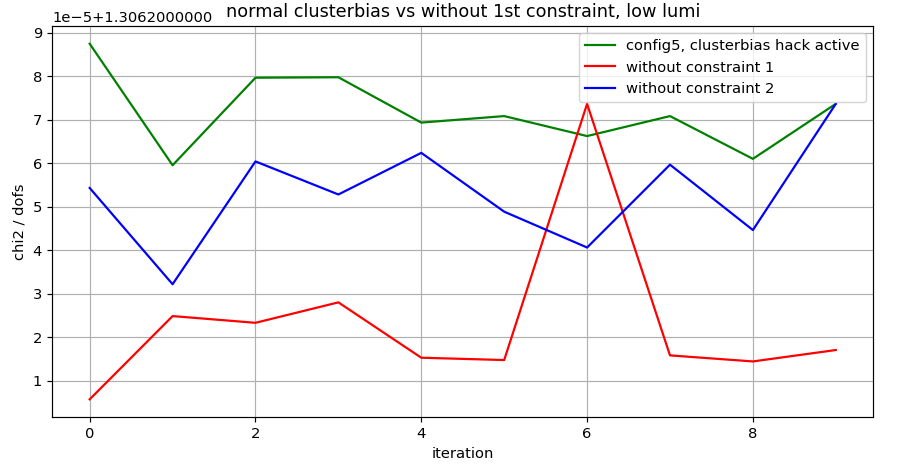
\includegraphics[width=0.8\textwidth]{plots/feb_6_2022/low_lumi_removed_constraints_vs_normal.png}
  \caption{impact of removing constraints from exisiting studies regarding chi2.}
  \label{fig:removeConst}
\end{figure}

We do want the least amount of constraints in the system so we also tested
the consequences of removing constraints from "config5".
The results are shown in figure \ref{fig:removeConst}.
The green curve shows the base config for comparison and in red the removal of the backlayer constraint in station 3 is shown. The blue curve shows the alignment results without the C-frame constraints.
The data samples used were from 2020 with the normal luminosity and an active clusterbias fix.
The selected track types are \textit{HighMomentumTTracks}(?) for 10000 events.
On the one hand we see an improvement in $\chi^2 / \text{dof}$ when removing these constraints individually even if it is only on a very small scale of $\num{1e-5}$. On the
other hand we see that the $\chi^2 / \text{dof}$ after the last iteration is the same for the base config and for the blue measurement. The constraint removed in the red measurement seems to have the most impact from what was tested but the peak in iteration 6 has no logical explanation. Additional analysis regarding constraint removal will be done in the future to analyse this phenomenon further.
Also the behavior of the not decreasing $\chi^2 / \text{dof}$ requires more testing.
What can be taken from this is that the removal of some constraints will help
the alignment but the cause of these abnormalities require more testing.
